   %%%%%%%%%%%%%%%%%%%
   %                 %
   %  capitolo2.tex  %
   %                 %
   %%%%%%%%%%%%%%%%%%%

   \chapter{Wetterich's non-perturbative FRG}
\noindent
The \emph{functional renormalization group} (FRG) is an approach to renormalization that combines the functional 
formulation of QFT with Wilson's ideas of renormalization. In the particular approach used in this thesis, introduced 
by \emph{Christof Wetterich}\cite{wetterichprimo}, one uses a scale dependent effective action, called 
\emph{effective average action}, usually indicated with $\Gamma_k$, where $k$ represents a coarse-graining scale, with physical dimension of a momentum.

The effective average action is 
a functional which interpolates between the classical bare action to be quantized, $S$, and the full quantum effective action $\Gamma$.
So, by definition, we have:
\begin{displaymath}
\left\{
\begin{array}{l}
 \Gamma_{k\rightarrow 0} = \Gamma\\
 \Gamma_{k\rightarrow \Lambda} = S
\end{array}
\right.
\end{displaymath}
Where $\Lambda$ is an ultraviolet cutoff, which represent the physical energy scale beyond which  QFT loses its validity.

If $\Lambda$ can be sent to $\infty$, then the quantum field theory is said UV complete.

Physically, $\Gamma_k$ is an effective action for average of fields, the average being taken over a volume $\approx k^{-d}$, 
so the degree of freedom with momenta greater than the coarse-graining scale $k$ are effectively integrated out. 

That renormalization procedure can be formulated directly for a continuum field theory, 
without the needs of a lattice regularization. 

In this chapters I will show how the exact evolution equation for the effective average action can be derived (\emph{i.e.} 
an equation for the derivative of $\Gamma_k$ with respect to $k$), I will discuss its proprieties  and I will mention the two
most common approximation schemes used in the literature that make that equation resolvable. 

\begin{figure}
\begin{center}
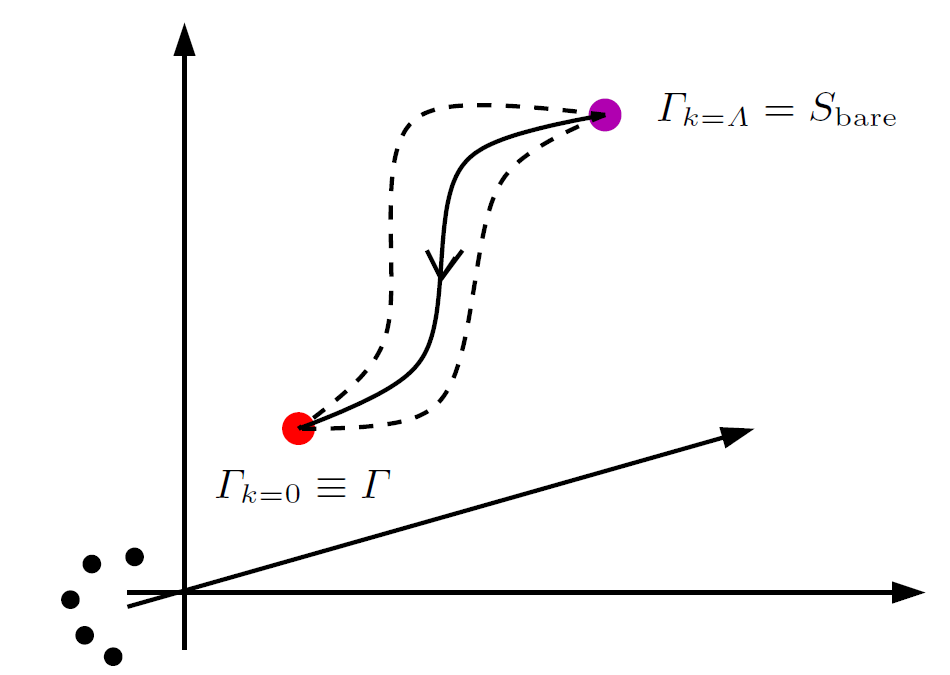
\includegraphics[scale=0.3]{Immagini/azionerunning.png}
\caption{A graphical representation of the renormalization group flow in the space of theories.  Each axis labels a different operator upon which the effective action depends. The functional renormalization group equation determines the evolution of the effective average action $\Gamma_k$, for a given initial condition $\Gamma_\Lambda = S$. A particular trajectory depends on the functional form of the regulator chosen, but all trajectories end at the full quantum action $\Gamma$ when $k\to0$.}
\label{fig:gammaflusso}
\end{center}
\end{figure}


\section{Derivation of the flow equation for $\Gamma_k(\phi_c)$}
The starting point of our treatment is the definition of a non-local regulator term to be added to the classical action:
\begin{equation}
 S_k[\phi] = S[\phi] + \Delta S_k[\phi]
\end{equation}
This term is, by definition,  quadratic in the fields, so it can be written in momentum space as:
\begin{equation}\label{essekappa}
 \Delta S_k[\phi] = \frac{1}{2} \int \frac{d^D q}{(2\pi)^D} \phi(-q)R_k(q)\phi(q)
\end{equation}
Physically, the functional $R_k(q)$ can be interpreted as a momentum-dependent correction to the mass term, and its definition
is the core of all Wetterich's method. According to that definition, we can write the scale dependent generating functional of the Euclidean $n$-point correlation functions $Z_k[J]$:
\begin{equation}\label{wdoppio}
 Z_k[J] \Def \exp \left( -\Delta S_k\left[\frac{\delta}{\delta J}\right] \right) Z_k[J] = \int_{\Lambda} \mathcal{D}\phi \e^{-S[\phi] -\Delta S_k[\phi] + J\cdot\phi}
\end{equation}
where I have defined the dot product between the fields and the classical source in the following way, in coordinate space:
\begin{equation}
 J\cdot\phi = \int d^Dx J_a (x)\phi^a(x)
\end{equation}
or, equivalently:
\begin{equation}
  J\cdot\phi = \int \frac{d^Dq}{(2\pi)^D} J_a (-q)\phi^a(q)
\end{equation}
in momentum space. The scale dependent generating functional of the connected Green function is defined analogously to what 
we've seen in the previous chapter, as the logarithm of $Z_k(\phi)$:
\begin{equation}\label{defW}
 W_k[J] := \ln(Z_k(\phi))
\end{equation}

The primary role of the regulator term is to suppress the contribution of lower modes (the ones inferior to $k$), 
leaving untouched the contribution of the higher ones. The choice of it is almost free. There are just three condition a function must satisfy in order to be coherently
taken as a regulator, conditions that ensure the evolution of $\Gamma_k$ will be well defined in the range $0\leq k\leq\Lambda$. 

As a function of $k$, the regulator function $R_k(q)$ must satisfy the following asymptotic conditions:
\begin{enumerate}
 \item 
 \begin{equation}\label{relazione1}
  \lim_{q^2/k^2 \to 0} R_k(q) > 0
  \end{equation}
       This condition implements the infrared regularization. It ensure that the exact propagator
       $G_k(q^2)$ doesn't diverge when $q^2\to 0$ at vanishing fields. 
       This usually happens because of the contribution of the massless modes, leading to infrared divergences problems. 
       So, that makes $R_k(q)$ an infrared regulator.
\item \begin{equation}\label{relazione2}
       \lim_{k^2/q^2 \to 0} R_k(q) = 0
      \end{equation}
        This condition means that, as it must happens, $Z_{k \to 0}[J] \to Z[J]$ 
       (and, consequently, $\Gamma_{k \to 0}[J] \to \Gamma[J]$), so in this limit the full quantum behavior is recovered.
\item \begin{equation}\label{relazione3}
\lim_{k^2 \to \Lambda^2} R_k(q) \rightarrow \infty
\end{equation}
     When $k$ approaches the ultraviolet cutoff $\Lambda$ the regulator terms causes an exponential suppression of the quantum 
     corrections in the path integral \eqref{wdoppio}, that becomes dominated by the stationary points of the classical action $S$. 
\end{enumerate}
Now we have all we need to derive the \emph{Wetterich equation} or, in other words, the \emph{flow equation for the effective average action}, 
which represent the central tool of the functional renormalization group.

First of all, I will define the \emph{effective average action} in a similar way to what I've done for the effective action in the previous chapter:
\begin{equation}\label{convessa}
 \Gamma_k[\phi_c] = \sup_J \left(\int J\phi_c - W_k[J]\right) - \Delta S_k[\phi]
\end{equation}
where I have also defined the \emph{classical field}:
\begin{equation}\label{otto}
 \phi_c = \langle \phi \rangle = \frac{\delta W_k[J]}{\delta J}
\end{equation}
It's important to note that, because of definition \eqref{otto}, if we define the source as fixed, the field will depend on the scale $k$ and 
\emph{viceversa}. Since later we'll want to study the effective average action as a functional of a fixed classical field, necessarily the classical
source $J$ will be a scale dependent quantity.
Another observation I want to remark is that, because of the terms $\Delta S_k(\phi_c)$, eq.\eqref{convessa} is not mathematically
a Legendre transformation, so $\Gamma_k$ (unlike $\Gamma$) is not necessarily convex. The convexity is obviously recovered in the limit $k\to0$.
\begin{figure}
\begin{center}
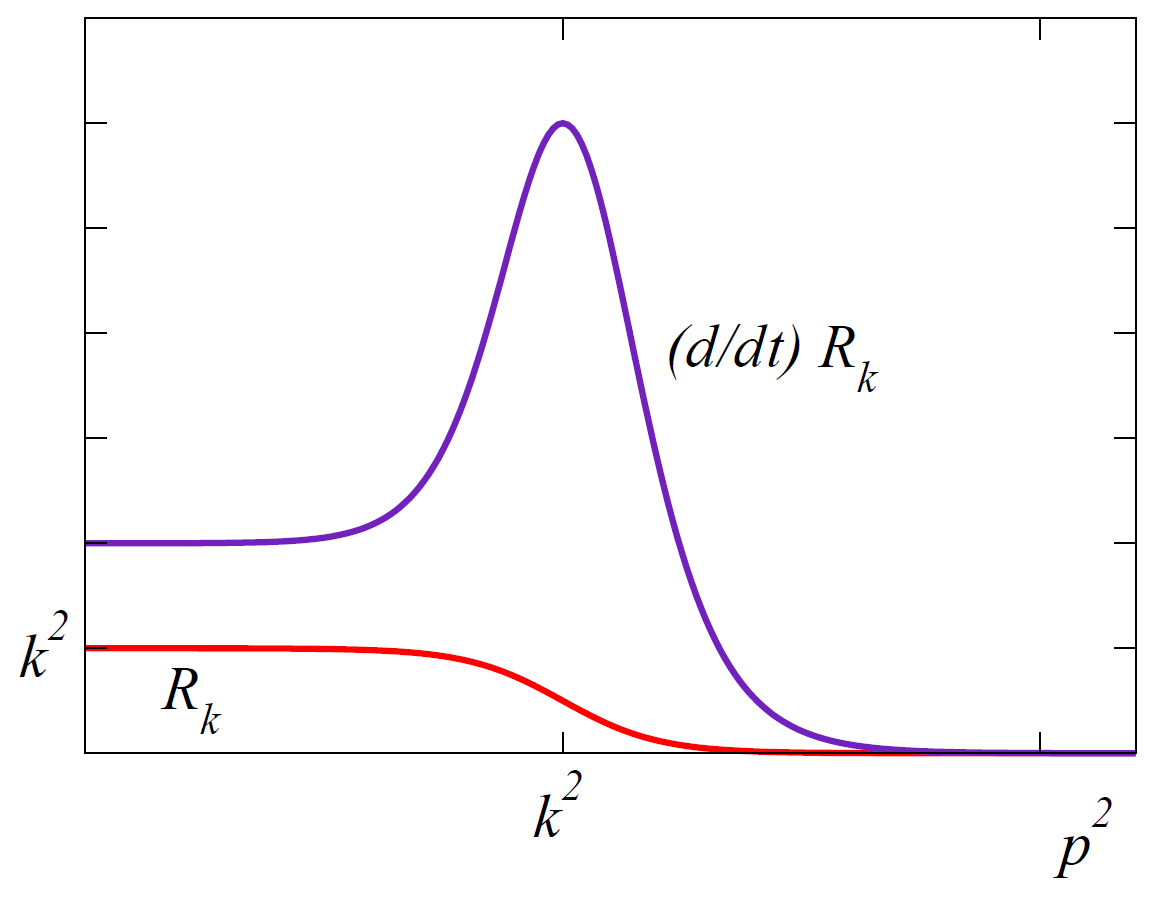
\includegraphics[scale=0.27]{Immagini/redrpunto.png}
\caption{The typical form of a regulator function $R_k$ as a function of $p^2$ (lower curve) and of its derivative $\partial_tR_k$. Due to its finite value for $p^2 \to 0$, the regulator provides for an IR regularization, while its derivative, due to the peaked form we can see plotted in the graph, implements the wilsonian idea of UV regularization by integrating out only fluctuations within a momentum shell near $p^2 \approx k^2$.}
\label{regolatore}
\end{center}
\end{figure}

Differentiating eq.\eqref{convessa} with respect to $k$ we obtain:
\begin{equation*}
 \partial_k \Gamma_k= \int d^D x\partial_kJ(x)\phi_c(x)- \partial_kW_k(J) - \int\frac{\partial W_k[J]}{\partial J(x)}\partial_kJ(x) - \partial_k \Delta S_k[\phi_c]
\end{equation*}
Because of definition \eqref{otto}, the first and the third terms cancel each other and we obtain:
\begin{equation}\label{flussogamma}
 \partial_k \Gamma_k= - \partial_kW_k[J] - \partial_k \Delta S_k[\phi_c]
\end{equation}
Here the derivative of $W[J]$ with respect to $k$ appears. This can be calculated differentiating eq.\eqref{defW} and using eq.\eqref{wdoppio}. The result is:
\begin{equation*}
 \partial_k W_k[J] = -\frac{1}{2}\int d^Dx \int d^Dy\partial_kR_k(x, y)G^{(2)}_k(y,x) - \partial_k\Delta S_k[\phi_c] =
\end{equation*}
\begin{equation}
 = - \frac{1}{2}\Tr(\partial_kR_kG_k^{(2)}) - \partial_k\Delta S_k[\phi_c] 
\end{equation}
where I used the definition of the scale dependent \emph{connected propagator} $G_k(q)$:
\begin{equation}
 G_k = \left( \frac{\delta^2 W_k}{\delta J \delta J}  \right)  =  \langle \phi\phi\rangle -  \langle \phi\rangle \langle\phi\rangle
\end{equation}
If we now substitute this result into eq.\eqref{flussogamma}, we obtain:
\begin{equation}
\partial_k\Gamma_k[\phi_c] = \frac{1}{2}\Tr\big(\partial_kR_kG_k^{(2)}\big)
\end{equation}
What remains to do, now, is to find an expression of the exact propagator in terms of $\Gamma_k$ and of the regulator $R_k$. First of all we notice that, 
because of eq.\eqref{flussogamma}, the quantum equation of motion receives a regulator modification:
\begin{equation}
 J(x) = \frac{\delta\Gamma_k[\phi_c]}{\delta\phi_c(x)} + (R_k\phi)(x)
\end{equation}
From this we have:
\begin{equation}
 \frac{\delta J(x)}{\delta\phi_c(y)} = \frac{\delta^2\Gamma_k[\phi_c]}{\delta\phi_c(x)\delta\phi_c(y)} + R_k(x,y)
\end{equation}
while, from eq.\eqref{otto}, we have:
\begin{equation}
 \frac{\delta\phi_c(y)}{\delta J(x')} = \frac{\delta^2W_k[J]}{\delta J(x')\delta J(y)} = G_k(y-x')
\end{equation}
So we have obtained the following important relation:
\begin{small}
\begin{equation}
 \frac{\delta J(x)}{\delta J(x')} = \delta(x - x') = \int d^D y\frac{\delta J(x)}{\delta \phi_c(y)}\frac{\delta \phi_c}{\delta J(x')} = \int d^D y\left(\frac{\delta^2 \Gamma_k[\phi_c]}{\delta \phi_c(x)\delta \phi_c(y)} + R_k(x,y) \right)G_k(y-x')
\end{equation}
\end{small}
Or, in other words:
\begin{equation}
 G_k(x - y) = \left(\frac{\delta^2 \Gamma_k[\phi_c]}{\delta \phi_c(x)\delta \phi_c(y)} + R_k(x,y)\right)^{-1}
\end{equation}
Collecting everything, we can finally obtain the celebrated \emph{Wetterich's equation}, that describes the flow of the 
effective average action:
\begin{equation}\label{wetterich}
 \dot{\Gamma}_k[\phi_c] \equiv \partial_t\Gamma_k[\phi_c] = \frac{1}{2}\Tr\left\{\partial_tR_k \left(\frac{\delta^2 \Gamma_k[\phi_c]}{\delta \phi_c(x)\delta \phi_c(y)} + R_k(x,y)\right)^{-1}\right\}
\end{equation}
For the sake of convenience, I have defined the adimensional parameter $t$, sometimes called RG time in the literature, in the following way:
\begin{equation}
 t := \ln \left(\frac{k}{\Lambda}\right), \ \ \ \ \ \ \ \ \ \ \ \ \partial_t := k \frac{d}{d k}
\end{equation}

The Wetterich's equation is the starting point of all our future investigations. Here I will spend some words on its proprieties:
\begin{figure}
\begin{center}
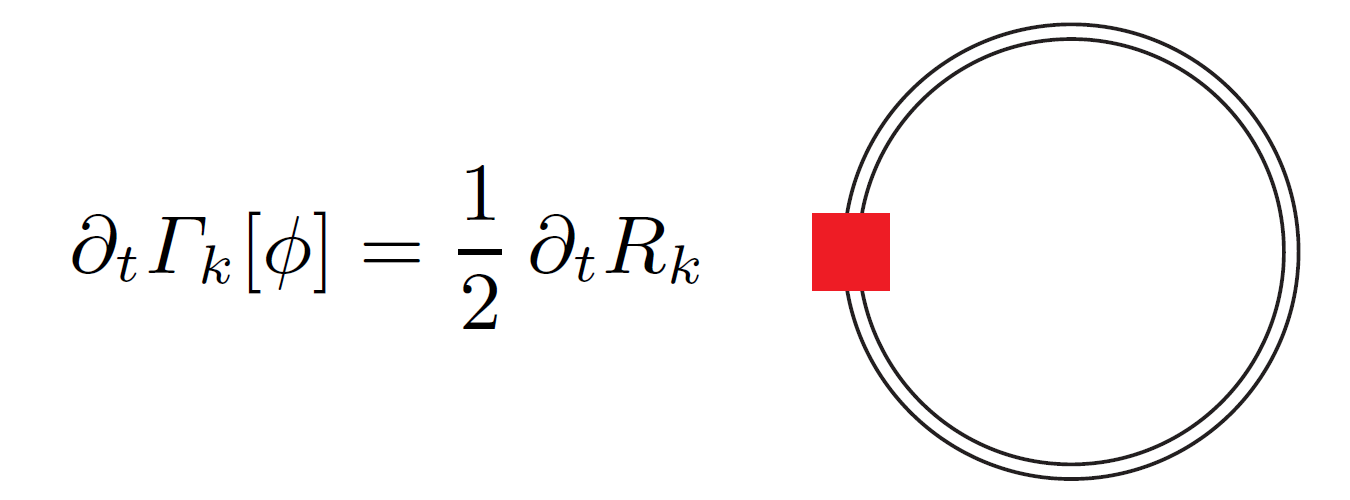
\includegraphics[scale=0.25]{Immagini/flussogamma.png}
\caption{A graphical representation of the Wetterich's equation. The flow of $\Gamma_k$ is given by a one-loop form, which involves the full propagator, represented here by a double line, and the operator $\partial_tR_k$, represented by afilled red box}
\label{fig:gammaflusso}
\end{center}
\end{figure}
\begin{enumerate}
\item This is a functional differential equation, so there are not functional integration to be performed (in contrast with eq.\eqref{wdoppio}).
\item The role of the regulator $R_k$ is twofold: its presence in the denominator of eq.\eqref{wetterich} ensures the infrared regularization, while its derivative $\partial_tR_k$ in the numerator ensures UV regularization, because its support lies on a smeared momentum shell near $p^2 \approx k^2$. This peaked structure of $\partial_tR$ implements nothing but the wilsonian idea of integrating momentum shell by momentum shell and implies that the flow is localized in momentum space. A typical form of a regulator and of its $t$ derivative is depicted in Fig.\ref{regolatore}
\item The Wetterich's equation has a one-loop structure, but it is nevertheless an exact equation, due to the presence of the exact propagator. This structure is the direct consequence of the fact that the regulator term we added to the classical action, $\Delta S_k$, is quadratic in the fields.
\end{enumerate}


\section{Approximations schemes}

The Wetterich's equation, despite its simple form, can't be solved exactly for an arbitrary $\Gamma_k$; that's simply because it
would be technically impossible to find an exact generic solution for a system of infinite coupled integro-differential equations.
So, some approximation on the effective action must be made.

In the following I will discuss the two main approximation method used in the literature: the \emph{vertex expansion} and the \emph{derivative expansion}.
These approximations don't rely on the smallness of a coupling parameter, so the method is, in essence, still  non perturbative. 
The mathematical results of making such approximations is to transform the Wetterich equation into a set of differential equations, 
sometimes much more easy to solve.



\subsection{Vertex expansion}
The vertex expansion approach was introduced and  extensively investigated by Tim R. Morris \cite{verticemorris} and it is widely used in the 
condensed matter physics community and also in low energy QCD studies. It is based upon a truncation of the effective average action in powers of the field:
\begin{equation}
 \Gamma_k[\phi_c] = \sum_{n = 0}^\infty = \frac{1}{n!}\int d^D x_1 \dots d^Dx_n \Gamma_k^{(n)}(x_1, \dots, x_n)\phi_c(x_1)\dots\phi_c(x_n)
\end{equation}
where I have indicated with $\Gamma_k^{(n)}$ the $n^{th}$ order functional derivative of $\Gamma_k$ with respect to the field.
By inserting this into the Wetterich's equation \eqref{wetterich} we obtain the flow equations for the vertex functions $\Gamma_k^{(n)}$, which
can be viewed as a differential FRG form of the Schwinger-Dyson equations.

It has been demonstrated that expanding the effective average action around the field corresponding to  the minimum of $\Gamma_k$ improves 
the convergence proprieties when one is interested in the behavior of the system near phase transitions \cite{verticefasi}.  

\subsection{Derivative Expansion}
In order to obtain approximate solutions of the flow equations, the other main strategy is the derivative expansion of the effective action.
That consists in expanding the effective average action in powers of the gradient of the field. 
This method is often applied to problems where one is interested in low momenta (or, equivalently, long wavelength) behavior,
or when the local structure is known to dominate.

It is the most used approximation technique in the literature and its convergence proprieties has been largely discussed (see, for example, \cite{verticefasi}). 

In this thesis this technique will be applied to the $O(N)$ model, so it will be extensively discussed in the following chapters.
For this reason, I will not spend much words about it now.

\section{Regulator dependence and optimization}
As we have seen, any explicit application of Wetterich's equations requires some approximation and every approximate solutions have a restricted domain of validity.  In addition to that, when approximations are made, the 
independence of physical observables from the choice of the regulator functional is lost. 

If we consider a family of regulators $R_k^{\alpha}(q)$ parametrized by $\alpha$, we are interested in find the particular value of $\alpha$
which minimizes the dependence of the observables of interest from $\alpha$ itself. This translates in the requirement:
\begin{equation}
 \left.\frac{d\mathcal{O}(\alpha)}{d\alpha}\right|_{\alpha = \alpha_{opt}} = 0
\end{equation}
where $\mathcal{O}$ is any physically interesting observable of the model (\emph{e.g.} the effective potential, a critical exponent, etc...).
This idea is called \emph{principle of minimum sensitivity} (PMS) \cite{altrolitim}.

\subsection{Example of regulators}
Various choice of the regulator functional have already been studied in great detail in the literature.
Here I will review the most common ones used and I will discuss the optimal parameter choice in the case of the evolution equation of the effective potential in 
the linear $O(N)$ model in the LPA (local potential approximation) of derivative expansion, which will be studied in depth in the following chapter of this thesis.
In general, because of issues due to numerical calculation, it is preferable to work with the dimensionless rescaled regulator, defined in the following way:
\begin{equation}
 r_k = \frac{R_k(q)}{Z_kq^2}
\end{equation}
where $Z_k$ is the wavefunction renormalization of the model, calculated in the configuration that minimizes the effective potential.
The dimensionless regulator results to be a function only of $q^2/k^2 \Def y$. For the sake of simplicity, I will discuss directly the rescaled regulators in the following.
\begin{enumerate}
 \item Exponential regulator\cite{powerlaw}:
      $$r_{exp}(y) = \frac{a}{\e^{cy^b} - 1}\ \ \ \ \ \  \ \ \ \ \ \ \ \ \ \ b\geq1$$
      In the linear $O(N)$ model treated with the LPA, the optimal parameter choice is $a = 1$, $c = \ln(2)$ and $b = 1.44$.
 \item Power Law regulator\cite{exp}:
      $$r_{pow}(y) = \frac{a}{y^b}$$
      with optimal choice $a = 1$ and $b = 2$.
 \item Litim regulator\cite{litim}:
      $$r_{Lit} (y) = a\left( \frac{1}{y^b} - 1\right)\theta(1-y)$$
      that is a continuous but not differentiable regulator with a compact support. It's one of the most widely used in the literature.
      The optimal choice for the parameters are $a = 1$ and $b = 1$.
 \item CSS regulator\cite{13}:
      $$r_{CSS}(y) = \frac{\exp[{cy_0^b}/({1 - hy_0^b})] - 1}{\exp[{cy^b}/({1 - hy^b})] - 1}\theta(1-hy^b)$$
      It's a very general regulator functional, that recovers all the other ones discussed here as special limits:
      \begin{itemize}
       \item Litim $$\lim_{c\to 0, h\to0} r_{CSS} = \frac{y_0^b}{1 - y_0^b}\left(\frac{1}{y^b} - 1\right) \theta (1 - y)$$
       \item Power Law       $$\lim_{c\to 0, h\to1} r_{CSS} = \frac{y_0^b}{y^b}$$
       \item Exponential $$\lim_{c\to 0, h\to1} r_{CSS} = \frac{\exp[y_0^b] - 1}{\exp[y^b] - 1}$$
      \end{itemize}
\end{enumerate}



\section{Application: the scalar model}
Now I will illustrate the capabilities of the functional renormalization group by a simple but highly 
nontrivial example: the scalar model in $D$ dimensions, described by the following bare action:
\begin{equation}
 S[\phi] = \int d^Dx\left[\frac{Z}{2}\partial^\mu\phi\partial_\mu\phi + V(\phi)\right]
\end{equation}
which now we are going to quantize.
\subsection{The effective potential}
The effective average action is: 
\begin{equation}
 \Gamma_k[\phi] = \int d^D x \left(\frac{Z_k}{2}\partial^\mu \phi \partial_\mu \phi + U_k(\rho) + \mathcal{O}(\partial^2)\right)
\end{equation}
where I have assumed that the effective potential is a function of the field modulus square $\rho = \phi^2/2$. 
Note also that, here and in the following, for the sake of brevity, I will indicate the classical field $\phi_c$ simply with $\phi$. 

I'll use as approximation scheme the derivative expansion in the  LPA' which is, together with LPA, one of the most widely used approximation in the literature.
It consists in keeping only a field independent (but scale dependent) coefficient in the kinetic term, unlike the simpler LPA which consider that term identically equal to one:
\begin{enumerate}
 \item $Z = 1\ \ \ \Longrightarrow$ LPA
 \item $Z = Z_k\ \  \Longrightarrow$ LPA'
\end{enumerate}
The running proper vertices and the Hessian will be calculated for a constant field $\phi_0$, the value which minimizes the effective potential:
\begin{equation}
 \phi(x) \approx \phi_0\ ;\ \ \ \ \ \ U_k\left(\frac{\phi_0^2}{2}\right) = 0
\end{equation}
This is enough if we want to have a first estimate of the functional form of the potential $U_k(\rho)$.

We chose the regulator function to be the \emph{Litim regulator}:
\begin{equation}\label{erre}
 R_k(p^2) = Z_k(k^2 - p^2)\theta(k^2 - p^2)
\end{equation}
\begin{equation}\label{errepunto}
 \dot{R}_k(p^2) = Z_k[(2 - \eta_k)k^2 + \eta_k p^2]\theta(k^2 - p^2)
\end{equation}
Where I have defined the \emph{running anomalous dimension} $\eta = -\dot{Z}_k/Z_k$.
The Hessian of the model, is given by the following expression:
\begin{equation}
 \Gamma_k^{(2)} [\phi, p^2] = Z_k p^2 + U_k^{(2)} (\rho)
\end{equation}

So, substituting it in the Wetterich equation in momentum space we obtain:
\begin{equation*}
 \partial_t U_k(\rho) = \frac{Z_k}{2}\int\frac{d^D p}{(2\pi)^D}\frac{(2 - \eta_k)k^2 + \eta_k p^2}{Z_kk^2 + U_k'(\rho) +  2\rho U_k''(\rho)}\theta(k^2 - p^2) =
\end{equation*}
\begin{equation}
 = Z_k v_D \int_0^{k^2} dp^2\frac{(2-\eta_k)k^2 - \eta_k p^2}{Z_k k^2 + U_k'(\rho) +  2\rho U_k''(\rho)}(p^2)^\frac{D-2}{2}
\end{equation}
where a spherical polar coordinate system was introduced and the spherical symmetry of the integrand used in order to separate the integration in $p$ to the one in the angular coordinates.

I have also defined, for the sake of brevity, the constant $v_D$, in the following way:
\begin{equation*}
 v_D^{-1} = 2^{D+1}\pi^\frac{D}{2}\Gamma\left(\frac{D}{2}\right)
\end{equation*}
The result is easily obtined after some manipulation. It is:
\begin{equation}
 \partial_tU_k(\phi) = \frac{4v_DZ_k(D -\eta_k +2)k^{D + 2}}{Z_k k^2 +  U_k'(\rho) +  2\rho U_k''(\rho)}
\end{equation}
Now it's useful to express the latter equation in terms of dimensionless quantities, so I will define an adimensional potential and an adimensional field 
modulus square, in the following way:
\begin{displaymath}
\left\{
\begin{array}{l}
\widetilde{\rho} = Z_k k^{2-D} \rho \\
u_k({\widetilde{\rho}}) = k^{-D} U_k(\widetilde{\rho})
\end{array}
\right.
\end{displaymath}
So, after some trivial algebraic manipulation, we obtain:
\begin{equation}
\dot{u}(\widetilde{\rho}) = -D  u_k(\widetilde{\rho}) +(D - 2 + \eta)\widetilde{\rho}\frac{\partial u_k(\widetilde{\rho})}{\partial \widetilde{\rho}} + \frac{\pi^{-\frac{D}{2}} (D- \eta_k +2)}{2^{D-1} \Gamma \left(\frac{D}{2}\right)(1 + u_k'(\widetilde{\rho}) + 2 \widetilde{\rho} u_k''(\widetilde{\rho}))}
\end{equation}
Where the following relation has been used:
\begin{equation}
\left.\frac{\partial}{\partial t} U_k(\widetilde{\rho})\right|_{\widetilde{\rho}} = \left.\frac{\partial}{\partial t} [k_Du_k(\widetilde{\rho})]\right|_{\widetilde{\rho}} = k^D\dot{u}(\widetilde{\rho}) + D k^D u_k(\widetilde{\rho})
\end{equation}

\subsection{Anomalous dimension}
To close our set of equation we need also the flow equation for $Z_k$ or, in other words, an explicit expression for the anomalous dimension $\eta_k = -\dot{Z_k}/Z_k$.
This can be easily obtained from the evolution equation of $\Gamma^{(2)}_k(\phi)$ in momentum space. By definition, the expression of $\Gamma_k^{2}(\phi)$ is:
\begin{equation}
{\Gamma}^{(2)}_k(\phi, p^2) = \frac{\delta^2}{\delta \phi(p)\delta\phi^*(p)}{\Gamma}_k(\phi)=Z_kp^2 + U^{(2)}_k(\phi)
\end{equation}
So we have:
\begin{equation}
 Z_k = \frac{1}{V_D}\left.\frac{\partial^2}{\partial p^2}\Gamma_k^{(2)}(\phi, p^2)\right|_{p^2=0}
\end{equation}
and, of course:
\begin{equation}\label{zetaanomala}
 \dot{Z}_k = \frac{1}{V_D}\left.\frac{\partial^2}{\partial p^2}\dot{\Gamma}_k^{(2)}(\phi, p^2)\right|_{p^2=0}
\end{equation}
Where $V_D$ is the $D$- dimensional volume where the system under investigation is confined.
So the starting point of our calculation is the evolution equation for $\Gamma^{(2)}_k$, which can be obtined differentiating
twice the Wetterich's with respect to the fields:
\begin{equation}\label{punto?}
 \dot{\Gamma}_k^{(2)}(\phi) = \frac{1}{2}\Tr\left\{ \dot{R_k}\frac{\delta^2 }{\delta\phi_a\delta\phi_b}\frac{1}{{\Gamma_k}^{(2)} + R_k}\right\} 
\end{equation}
In order to calculate the second functional derivative of the exact propagator:
\begin{equation}
 G_k = \frac{1}{{\Gamma_k}^{(2)} + R_k}
\end{equation}
we use the well known formula for the derivative of a martix knowing its inverse:
\begin{equation}
 \frac{\partial}{\partial x} M^{-1} = - M^{-1}\left(\frac{\partial}{\partial x} M \right) M^{-1}
\end{equation}
And, for the second order derivative:
$$\frac{\partial^2}{\partial x\partial y} M^{-1} = $$
$$M^{-1}\left(\frac{\partial}{\partial x} M \right)M^{-1}\left(\frac{\partial}{\partial y} M \right) M^{-1} + M^{-1}\left(\frac{\partial}{\partial y} M \right)M^{-1}\left(\frac{\partial}{\partial x} M \right) M^{-1} -  M^{-1}\left(\frac{\partial^2}{\partial x\partial y} M \right) M^{-1}$$
So the second functional derivative of the exact propagator is, in coordinate space:
$$ \frac{\delta^2G_k(x_1, x_2)}{\delta \phi(x) \delta \phi(y)} = {G}_k(x_1,  x_3) \left[ 2\frac{\delta {\Gamma^{(2)}}(x_3, x_4)}{\delta \phi(x)}{G_k{(x_4, x_5)}} \frac{\delta {\Gamma_k^{(2)}}(x_5,  x_6)}{\delta \phi(y)} - \frac{\delta^2{\Gamma_k^{(2)}}(x_3, x_6)}{\delta \phi(x) \delta \phi(y)}\right] {G}_k({x_6, x_2})$$
So the trace in \eqref{punto?} becomes:
\begin{equation}
\frac{1}{2}\Tr\left\{ \dot{R_k}\frac{\delta^2 }{\delta\phi_a\delta\phi_b}\frac{1}{{\Gamma_k}^{(2)} + R_k}\right\} = 
\end{equation}
\begin{equation}
 = \left[ {G^{x_1 x_3}}_k \left(\frac{\delta {\Gamma^{(2)x_3 x_4}}_k}{\delta \phi(x)}{G^{x_4x_5}}_k \frac{\delta {\Gamma^{(2)x_5 x_6}}_k}{\delta \phi(y)} - \frac{1}{2}\frac{\delta^2{\Gamma^{(2)x_3x_6}}_k}{\delta \phi(x) \delta \phi(y)}\right) {G^{x_6x_2}}_k \right]{\dot{R_k}^{x_2 x_1}}\equiv A - \frac{1}{2}B
\end{equation}
Where I have used the generalized index notation: the $x_i$ are spacetime coordinate and the integration over repeated index is understood.
I will resolve the two integral separatly. The first one is:
\begin{equation}
\int \prod_{j=1}^6 dx_j G_k(x_3 - x_1) \frac{\delta {\Gamma^{(2)}}_k(x_3, x_4)}{\delta \phi(x)}{G_k(x_5 - x_4)} \frac{\delta {\Gamma^{(2)}(x_5, x_6)}_k}{\delta \phi(y)} G_k(x_2 - x_6)\dot{R_k}(x_1 - x_2) 
\end{equation}
We perform the calculation in momentum space so, we need the momentum-space expression of the quantities in \eqref{p}:
\begin{displaymath}
\left.
\begin{array}{l}
G_k (x_3-x_1) = \int \frac{d^Dq_1}{(2\pi)^D}  \widetilde{G}_k(q_1) e^{i(x_3-x_1)q_1}\\ \\
G_k (x_5-x_4) = \int \frac{d^Dq_2}{(2\pi)^D}  \widetilde{G}_k(q_2) e^{i(x_5-x_4)q_2}\\ \\
G_k (x_2-x_6) = \int \frac{d^Dq_3}{(2\pi)^D}  \widetilde{G}_k(q_3) e^{i(x_2-x_6)q_3}\\ \\
\Gamma^{(3)} (x, x_3, x_4) = \int \frac{d^Dp_1}{(2\pi)^D}\int \frac{d^Dp_2}{(2\pi)^D}\int \frac{d^Dp_3}{(2\pi)^D} \widetilde{\Gamma}^{(3)} \delta (p_1 + p_2 + p_3) e^{ip_1x}e^{ip_2x_3}e^{ip_3x_4}\\ \\	
\Gamma^{(3)} (y, x_5, x_6) = \int \frac{d^Dp'_1}{(2\pi)^D}\int \frac{d^Dp'_2}{(2\pi)^D}\int \frac{d^Dp'_3}{(2\pi)^D} \widetilde{\Gamma}^{(3)} \delta (p'_1 + p'_2 + p'_3) e^{ip'_1y}e^{ip'_2x_5}e^{ip'_3x_6}\\ \\
 \dot{R_k} = [2k^2 Z_k + \dot{Z}_k (k^2 - q^2)]\theta(k^2 - q^2)\\ \\
\end{array}
\right.
\end{displaymath}
Performing the integrations, the following constraints on the momenta are found:
\begin{center}
\begin{tabular}{cc}
$q_1 = q$ & $p_1 = p_1$\\
$q_3 = q$ & $p_1' + p_1 + q$\\
$p_2 = q$ & $p_2 = q$\\
$q_2 = -p_3$ & $p'_2 = -q$\\
$p_1' = q_2$ & $p_3 = -p_1 - q$\\
$p_2' = -q$ & $p_3' = -p_1$
\end{tabular}
\end{center}
After performing a Fourier transform, in order to express the result in momentum space, the following 
expression for the $A$ integral is obtained:
\begin{equation}
 A(p) = V_D\int \frac{d^Dq}{(2\pi)^D}\int\frac{d^Dp}{(2\pi)^D}G_k(q)\Gamma^{(3)}_k(p, q, -p - q)G_k(p+q)\Gamma^{(3)}_k(-p,-q, p+q)G_k(q) \dot{R}_k(q)
\end{equation}
In a similar way the integral $B$ can be evaluated, here I will just state the result:
\begin{equation}
B(p) = V_D \int \frac{d^Dq}{(2\pi)^D} \int\frac{d^Dp}{(2\pi)^D}G_k(q)\Gamma_k^{(4)}(p,-p,q,-q)G_k(q)\dot{R}_k(q)
\end{equation}
These two integrals have an immediate graphical interpretation in terms of two $1$-loop Feynmann diagrams, which I reported in Fig.\ref{fig:grafoA} and in Fig.\ref{fig:grafoB}.
\begin{figure}
\begin{center}
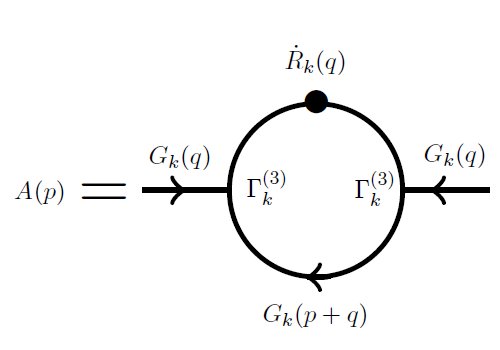
\includegraphics[scale=0.55]{Immagini/grafoA.png}
\caption{Graphical representation of the $A$ integral.}
\label{fig:grafoA}
\end{center}
\end{figure}
Now I will neclet the momentum dependence of the proper vertices, assuming:
$$\Gamma_k^{(3)} \approx 6\sqrt{\rho} U_k''(\rho) + 2\rho^{3/2} U_k'''(\rho)$$
$$\Gamma_k^{(4)} \approx 3\sqrt{\rho} U_k''(\rho) + 12\rho U_k'''(\rho)+ 4\rho^2 U_k''''(\rho)$$

This approximation on the vertices implies the $p$ independence of the $B$ graph, so recalling eq.\eqref{zetaanomala}, 
We come to the conclusion that this one has not influence on the flow equation for $Z_k$. So, putting all the elements
together, we come to the expression:
\begin{equation}\label{241}
 \dot{{Z_k}} =  \left({\Gamma}_k^{(3)}\right)^2 \int \frac{d^Dq}{(2\pi)^D} {G}^2_k(q) \dot{{R}}_k(q)\frac{\partial^2}{\partial p^2}\Big[{G}_k(p + q)\Big]_{p=0}
\end{equation}
In order to simplify the procedure, I will use the identity:
\begin{equation}
 \frac{\partial^2}{\partial p^2}\Big[{G}_k(p + q)\Big]_{p=0} = \frac{\partial^2}{\partial q^2}\Big[{G}_k(q)\Big]
\end{equation}
Now all we have to do is to calculate explicitly the derivative of the exact propagator:
\begin{equation}
\frac{\partial^2}{\partial q^2} \left( Z_k q^2 + U'_k(\rho) + 2\rho U_k''(\rho) + Z_k(k^2 - q^2)\theta(k^2 - q^2)\right)^{-1}
\end{equation}
The Heaviside $\theta$ function allows us to rewrite the preceding expression as a sum of two terms, in the following way:
\begin{equation}
\frac{\partial^2}{\partial q^2} \left(\frac{\theta(k^2 - q^2)}{Z_kk^2 + U'_k(\rho) + 2\rho U_k''(\rho)} +\frac{\theta(q^2 - k^2)}{Z_kq^2 + U'_k(\rho) + 2\rho U_k''(\rho)}\right)
\end{equation}
Performing the first derivative:
\begin{small}
\begin{equation*}
\frac{\partial}{\partial q^\mu}\Big[{G}_k(q)\Big] -\frac{2q_\mu\delta (k^2 - q^2)}{Z_kk^2 + U'_k(\rho) + 2\rho U_k''(\rho)} + \frac{2q_\mu\delta (q^2 - k^2)}{Z_kq^2 + U'_k(\rho) + 2\rho U_k''(\rho)} + \theta(q^2 - k^2) \frac{\partial}{\partial q^\mu}\frac{1}{Z_kq^2 + U'_k(\rho) + 2\rho U_k''(\rho)}
\end{equation*}
\end{small}
The first and the second terms cancel each other, so we have:
\begin{equation}
\frac{\partial}{\partial q^\mu}G_k(q) = - \frac{2q_\mu Z_k\theta(q^2 - k^2)}{\big(Z_k q^2 + U'_k(\rho) + 2\rho U_k''(\rho)\big)^2}
\end{equation}
and, performing the second derivative, we obtain the result:
\begin{equation}
\frac{\partial^2}{\partial q^2}\Big[{G}_k(q)\Big] = 2Z_k\left[ 4\frac{Z_kq^2\theta(q^2 - k^2)}{(Z_kq^2 + U'_k(\rho) + 2\rho U_k''(\rho))^3} - \frac{\theta(q^2 - k^2) + 2q^2 \delta(q^2 - k^2)}{(Z_kq^2 + U'_k(\rho) + 2\rho U_k''(\rho))^2} \right] 
\end{equation}
If we now substitute what we have found in equation \eqref{241} we have, recalling the definition of the Litim optimized regulator \eqref{erre},\eqref{errepunto},
that the terms containing the theta functions don't contribute to the integral, because their support is disjoint from the support of 
the theta function in the definition of $\dot{R}_k(q)$.
\begin{figure}
\begin{center}
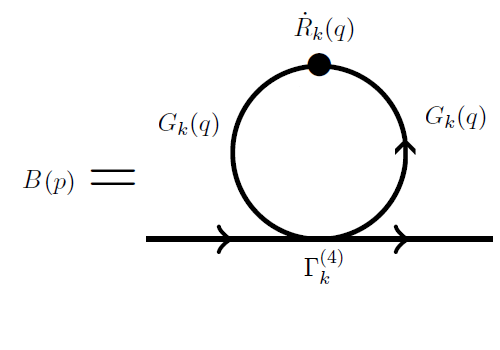
\includegraphics[scale=0.55]{Immagini/grafoB.png}
\caption{Graphical representation of the $B$ integral.}
\label{fig:grafoB}
\end{center}
\end{figure}

So, substituting this result in eq.\eqref{241} and recalling that $\delta(k^2 - q^2)\theta(k^2 - q^2)  = 1/2\delta(k^2 - q^2)$, after some trivial algebrical manipulation, we come to the following expression for the anomalous dimension:
\begin{equation}
  \eta_k = \left.\frac{32 v_D Z_k k^{D + 2}\Big[9\rho\big(U_k''(\rho)\big)^2+ 6 \rho^2 U_k''(\rho)U_k'''(\rho)+ \rho^{3} \big(U_k'''(\rho)\big)^2\Big]}{(Z_kk^2 + U'_k(\rho) + 2\rho U_k''(\rho))^4}\right|_{\rho = \rho_0}
\end{equation}
Where I have named $\rho_0$ the field modulus square at the potential minimun.
Now we should express the latter expression in terms of dimensionless quantities, so I recall the definitions of the adimensional potential and of the adimensional field modulus square:
\begin{displaymath}
\left\{
\begin{array}{l}
\widetilde{\rho} = Z_k k^{2-D} \rho \\
u_k({\widetilde{\rho}}) = k^{-D} U_k(\widetilde{\rho})
\end{array}
\right.
\end{displaymath}
So we obtain:
\begin{equation}
\eta_k = \frac{2^{4-D} \pi ^{-\frac{D}{2}} \left(3 \widetilde{\rho} u_k''(\widetilde{\rho} ) +\rho ^2 u_k'''(\widetilde{\rho} )\right)^2}{\rho  \Gamma \left(\frac{D}{2}\right) (1 + 2 \widetilde{\rho} u_k''(\widetilde{\rho}))^4}
\end{equation}
where all the quantities are calculated at the potential minimum.











